\chapter{Desarrollo del Sistema.}\label{sec:Desarrollo}

\paragraph{}En este capítulo vamos a conectar el uso teórico del entorno de desarrollo
mostrado en el capítulo \ref{sec:GuiaDeUso}, con el diseño software y la arquitectura de
la aplicación meteorológica del capítulo \ref{sec:AplicacionMeteorologica}. Lo haremos
explicando cómo hemos desarrollado varias tareas.

\section{Planificación del Sprint y tablón Kanban.}

\paragraph{}Como en cualquier desarrollo lo primero es planificar. A continuación se
muestran unas tablas Kanban con las tareas del sprint que vamos a explicar cómo se
han desarrollado.

\begin{table}[H]
\begin{center}
\begin{tabular}{| p{0.3\textwidth} | p{0.3\textwidth} | p{0.3\textwidth} |}
    \hline
    \multicolumn{3}{|c|}{Equipo de software de sistema} \\
    \hline
    To Do & In Progress & Done \\
    \hline
    &  & Lanzar automáticamente la aplicación al inicio. \\
    Generación de imagen de disco con características de debug y prueba en hardware. & & \\
    \hline
    \hline
    \multicolumn{3}{|c|}{Equipo de UI/UX} \\
    \hline
    To Do & In Progress & Done \\
    \hline
    Adecuación de la hora al huso horario de la localización. &  & \\
    \hline
\end{tabular}
\caption{Tablón Kanban}
\label{tab:Kanban}
\end{center}
\end{table}

\paragraph{}Teniendo claras las tareas de este sprint, vamos a proceder a realizarlas
y a documentar el proceso.

\section{Generación de imagen de disco con características de debug y prueba en hardware.}

\paragraph{}Esta prueba consiste en comprobar las características de debug en la
Raspberrry Pi, dichas características incluyen paquetes y configuraciones que no deben
estar presentes en producción pero que representan una ventaja a la hora de depurar.
Para esta prueba sólo vamos a necesitar el entorno de Yocto.

\paragraph{}Comenzamos abriendo con una terminal el directorio del entorno Yocto,
suponiendo que ya tengamos el entorno instalado. Aplicamos los cambios pertinentes
en el entorno para habilitar la posibilidad de incluir las características de depuración
con un argumento en el script de build.sh. Los cambios se pueden ver en forma de parche
en el siguiente cuadro:

\begin{lstlisting}[style=consola]
    diff --git a/build.sh b/build.sh
    index 4ab039b..fed2664 100755
    --- a/build.sh
    +++ b/build.sh
    @@ -8,6 +8,7 @@ __verbose=
     __bitbake_cmd=
     __only_shell=
     __wifi_settings_interactive=
    +__debug=
     while (( $# )); do
         case ${1,,} in
             -v|--verbose)
    @@ -26,6 +27,9 @@ while (( $# )); do
             -wi|--wifi-interactive)
                 __wifi_settings_interactive=1
                 ;;
    +        -d|--debug)
    +            __debug=":${repoPath}/debug.yml"
    +            ;;
             -h|--help)
                 print_help
                 exit 0
    @@ -80,15 +84,15 @@ fi

     if [ -n "${__only_shell}" ]
     then
    -    kas shell -E "${CONF_FILE}"
    +    kas shell -E "${CONF_FILE}${__debug}"
         exit 0
     fi

     ###Enable option for only start
     if [ -z "${__bitbake_cmd[*]}" ]
     then
    -    time kas build "${CONF_FILE}"
    +    time kas build "${CONF_FILE}${__debug}"
     else
         echo "Executing command: ${__bitbake_cmd[*]}"
    -    time kas shell "${CONF_FILE}" -c "${__bitbake_cmd[@]}"
    +    time kas shell "${CONF_FILE}${__debug}" -c "${__bitbake_cmd[@]}"
     fi
    diff --git a/debug.yml b/debug.yml
    new file mode 100644
    index 0000000..5baec50
    --- /dev/null
    +++ b/debug.yml
    @@ -0,0 +1,6 @@
    +header:
    +  version: 8
    +
    +local_conf_header:
    +  debug_features: |
    +    EXTRA_IMAGE_FEATURES += "debug-tweaks"
\end{lstlisting}

\paragraph{}Con los cambios realizados, abrimos una terminal e introducimos las siguientes
sentencias:

\begin{lstlisting}[style=consola, numbers=left]
    # Vamos realizar una primera compilacion para generar todas las tools del SDK
    $ ./build.sh --debug -wi

    # Introducimos los datos de nuestra red Wi-Fi.
    # Esperamos a que termine, esto puede durar varias horas

    $ ./getImageReady2Flash.sh
\end{lstlisting}

\paragraph{}Después de eso introducimos una tarjeta de memoria en el ordenador, y
suponiendo que la tarjeta es detectada como el dispositivo ``/dev/sdb'', realizamos
las siguientes operaciones:

\paragraph{}\textbf{Nota:} Comprueba cual es el dispositivo que asigna tu ordenador a la tarjeta
de memoria, usar un dispositivo incorrecto podría conllevar la pérdida de datos
importantes.

\begin{lstlisting}[style=consola, numbers=left]
    # Umount de las particiones de la uSD
    $ sudo umount /dev/sdb*

    $ sudo dd if=disk.img of=/dev/sdb bs=4M
    $ sync
\end{lstlisting}

\paragraph{}Ya estaríamos listos para extraer la memoria, colocarla en la ranura de
la Raspberry Pi y encenderla.

\paragraph{}Una vez encendida la Raspberry Pi, esta se conectará a internet mediante
el puerto ethernet o bien mediante Wi-Fi si hemos configurado bien las configuraciones.
Para comprobar que hemos activado bien las características de depuración intentaremos
abrir una sesión ssh con el usuario ``root'' sin contraseña con:

\begin{lstlisting}[style=consola, numbers=left]
    $ ssh root@raspberrypi3.local
\end{lstlisting}

\paragraph{}Si obtenemos el acceso, la prueba habrá sido satisfactoria.

\section{Adecuación de la hora al huso horario de la localización.}

\paragraph{}Vamos a mezclar todos los entornos para esta tarea, desarrollando, probando
en local y el hardware. Lo primero es ir al entorno de desarrollo Yocto. Una vez allí,
abrir una terminal y realizar las siguientes operaciones:

\begin{lstlisting}[style=consola, numbers=left]
    # Vamos realizar una primera compilacion para generar todas las tools del SDK
    $ ./build.sh --debug

    # Abrimos una terminal interactiva
    $ ./build.sh --debug --shell

    # Incluimos el codigo del entorno Flutter en el eSDK
    $ devtool modify rpi-weather
\end{lstlisting}

\paragraph{}Con esto tendremos el código del entorno de desarrollo Flutter descargado
en la carpeta raspberrypi3/workspace/sources. Podremos por tanto, abrir una instancia
de \Gls{vscode} en la carpeta con las fuentes de Flutter.

\paragraph{}Una vez abierta la instancia de \Gls{vscode} podremos seguir las instruciones
del capítulo \href{sec:ManualDeInstalacion}{Manual de Instalación}. Con las dependencias
descargadas y el entorno preparado, podremos empezar a desarrollar.

\begin{figure}[H]
    \centering
    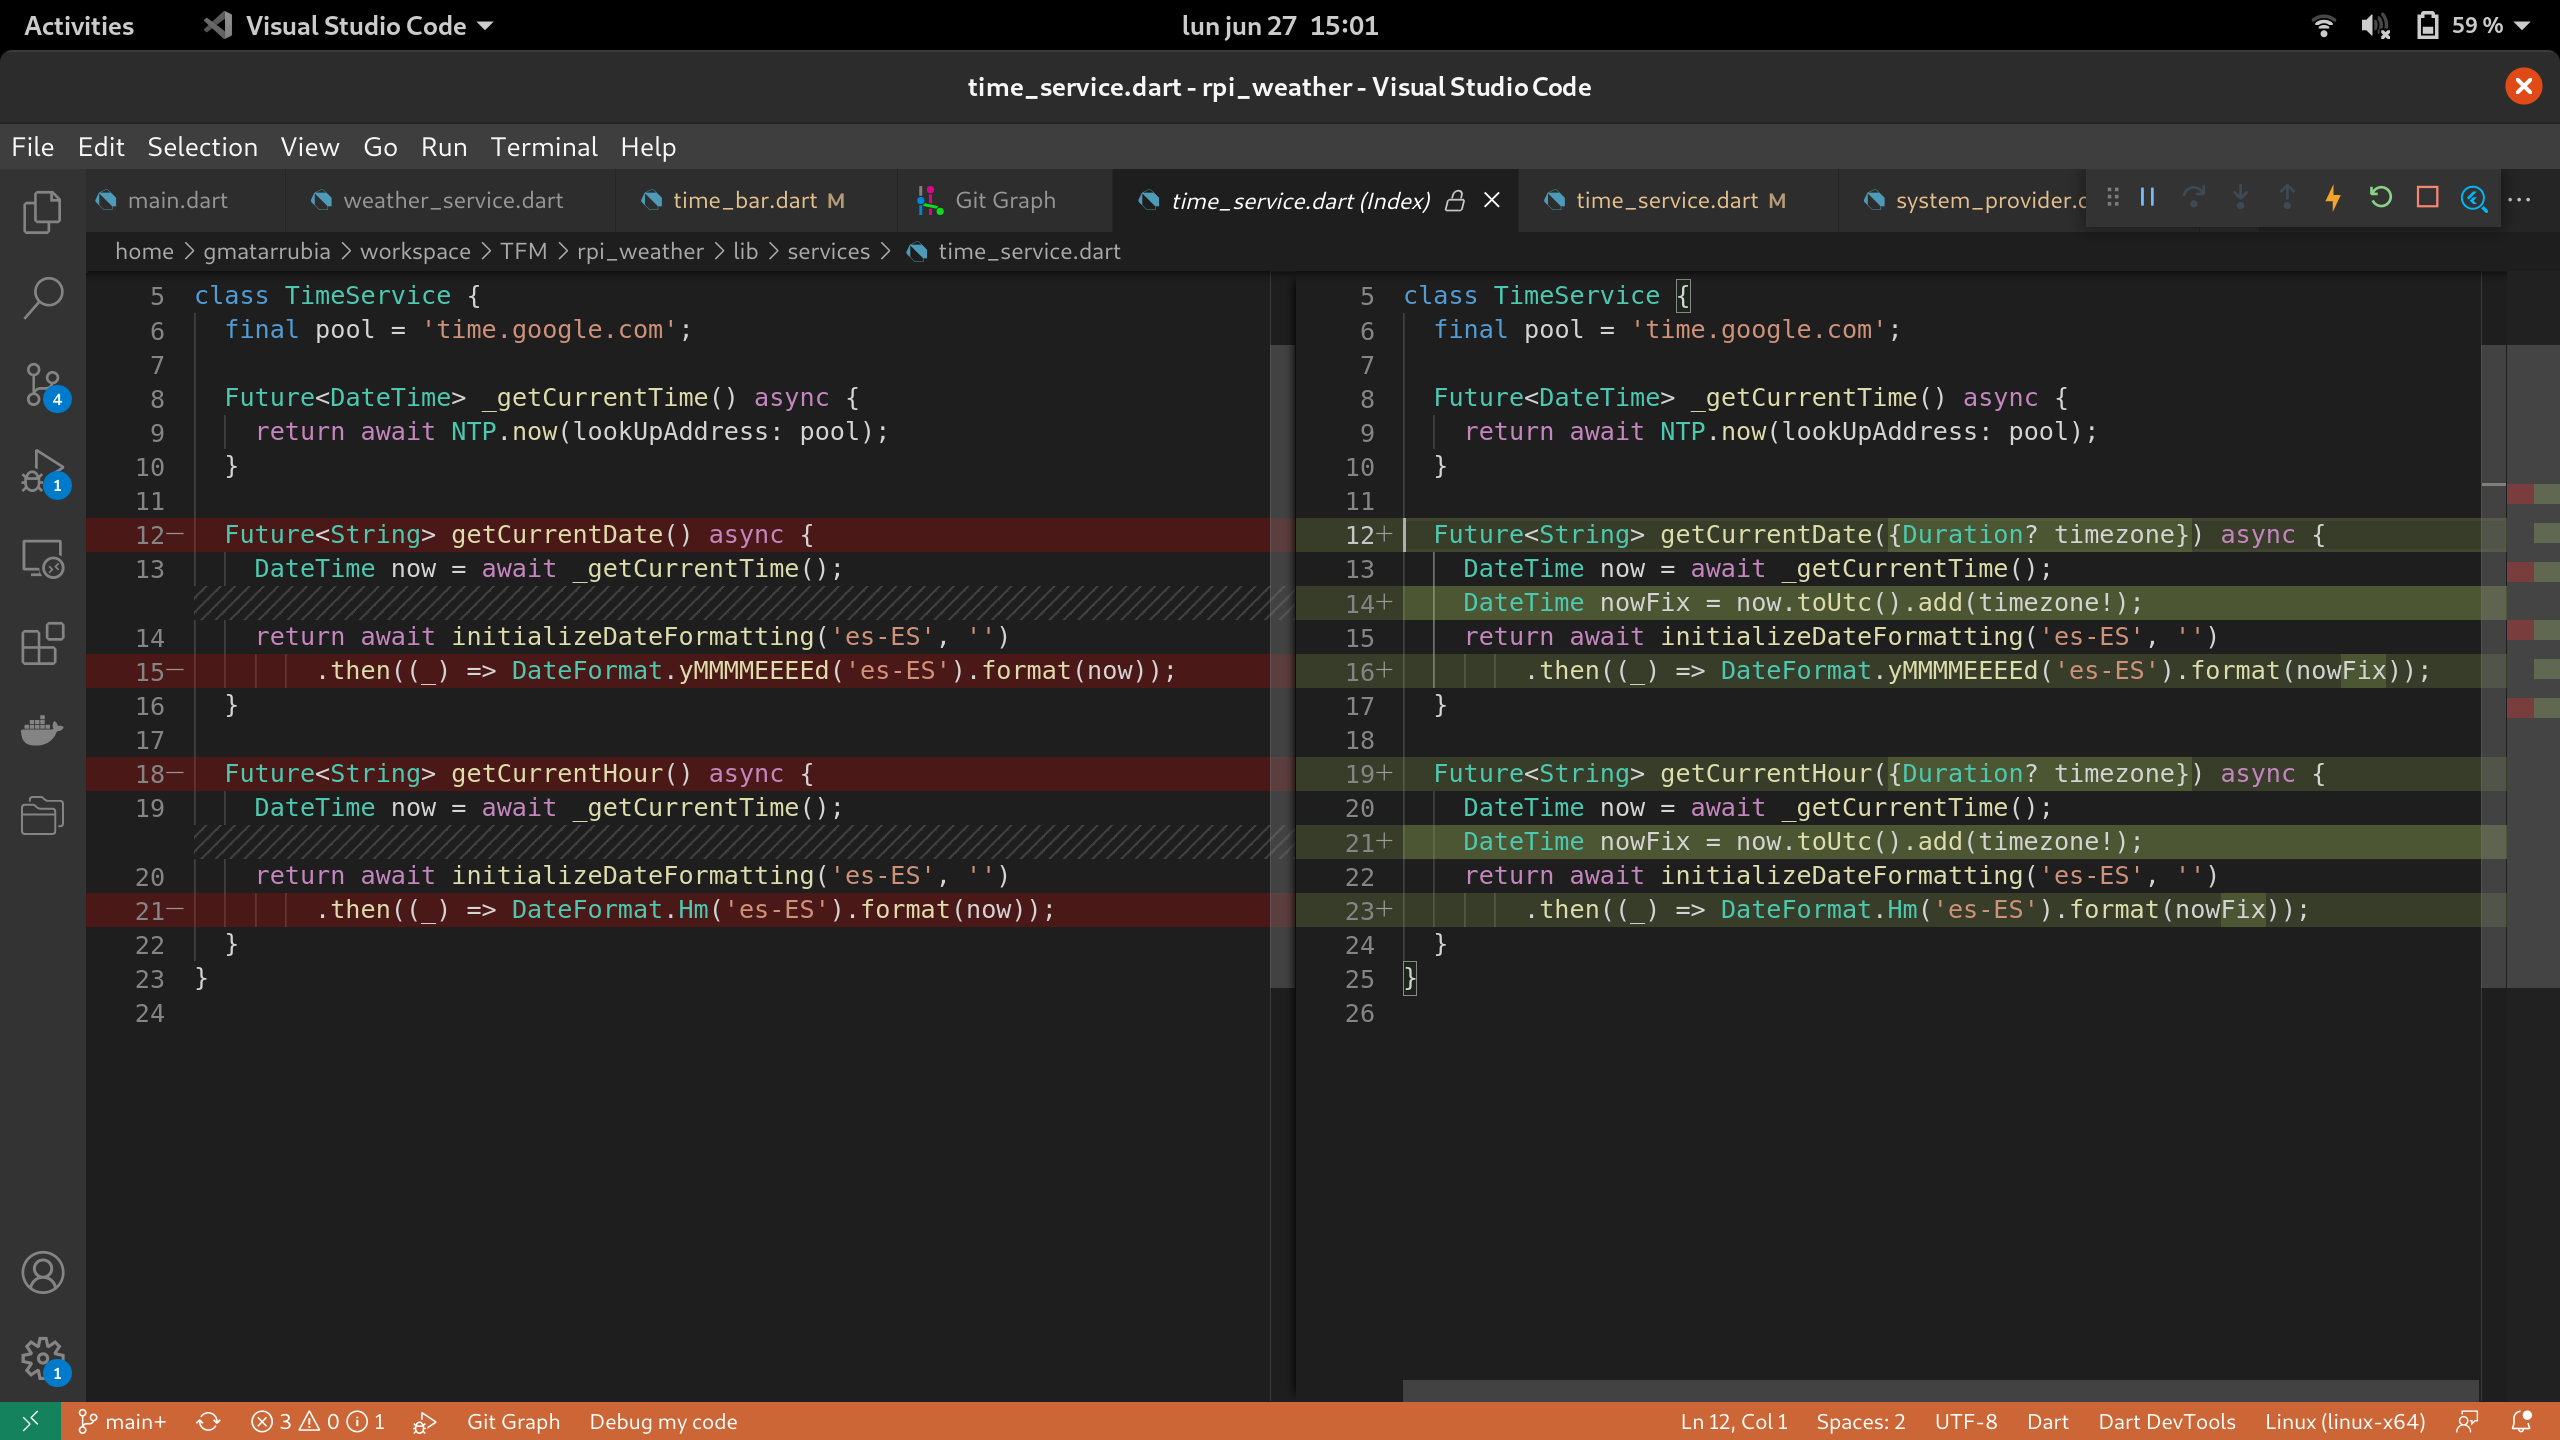
\includegraphics[width=0.95\textwidth]{imgs/dev1}
    \caption[Diff de los cambios.]{Diff de los cambios.}
    \label{imgs:diff-code}
\end{figure}

\paragraph{}Cómo podemos ver en la imágen \ref{imgs:diff-code} se han realizado algunos
cambios en el código. Y la imagen muestra la comparativa entre del archivo de antes y de después
de los cambios.

\paragraph{}Iremos compilando y depurando como es habitual en el desarrollo de cualquier
característica. Cuando quedemos satisfechos con los resultados y nos cercioremos en la
medida de lo posible de que no haya bugs, probaremos la aplicación en el hardware.

\paragraph{}\textbf{Nota:} Es importante haber preparado previamente la imagen del sistema
con las características de debug.

\paragraph{}Antes del despliegue tendremos que loguearnos por ssh en la Raspberry Pi 3
y para el servicio que corre la aplicación flutter.

\begin{lstlisting}[style=consola, numbers=left]
    $ systemctl stop flutter-app.service
\end{lstlisting}

\paragraph{}También tendremos que recuperar la terminal de la shell interactiva que habíamos
abierto interactivamente. Con esa terminal, compilaremos la aplicación con el engine
embebido y luego realizamos el despliegue con los sigueintes comandos:

\begin{lstlisting}[style=consola, numbers=left]
    $ devtool build rpi-weather
    $ devtool deploy-target rpi-weather root@<IP>
\end{lstlisting}

\begin{figure}[H]
    \centering
    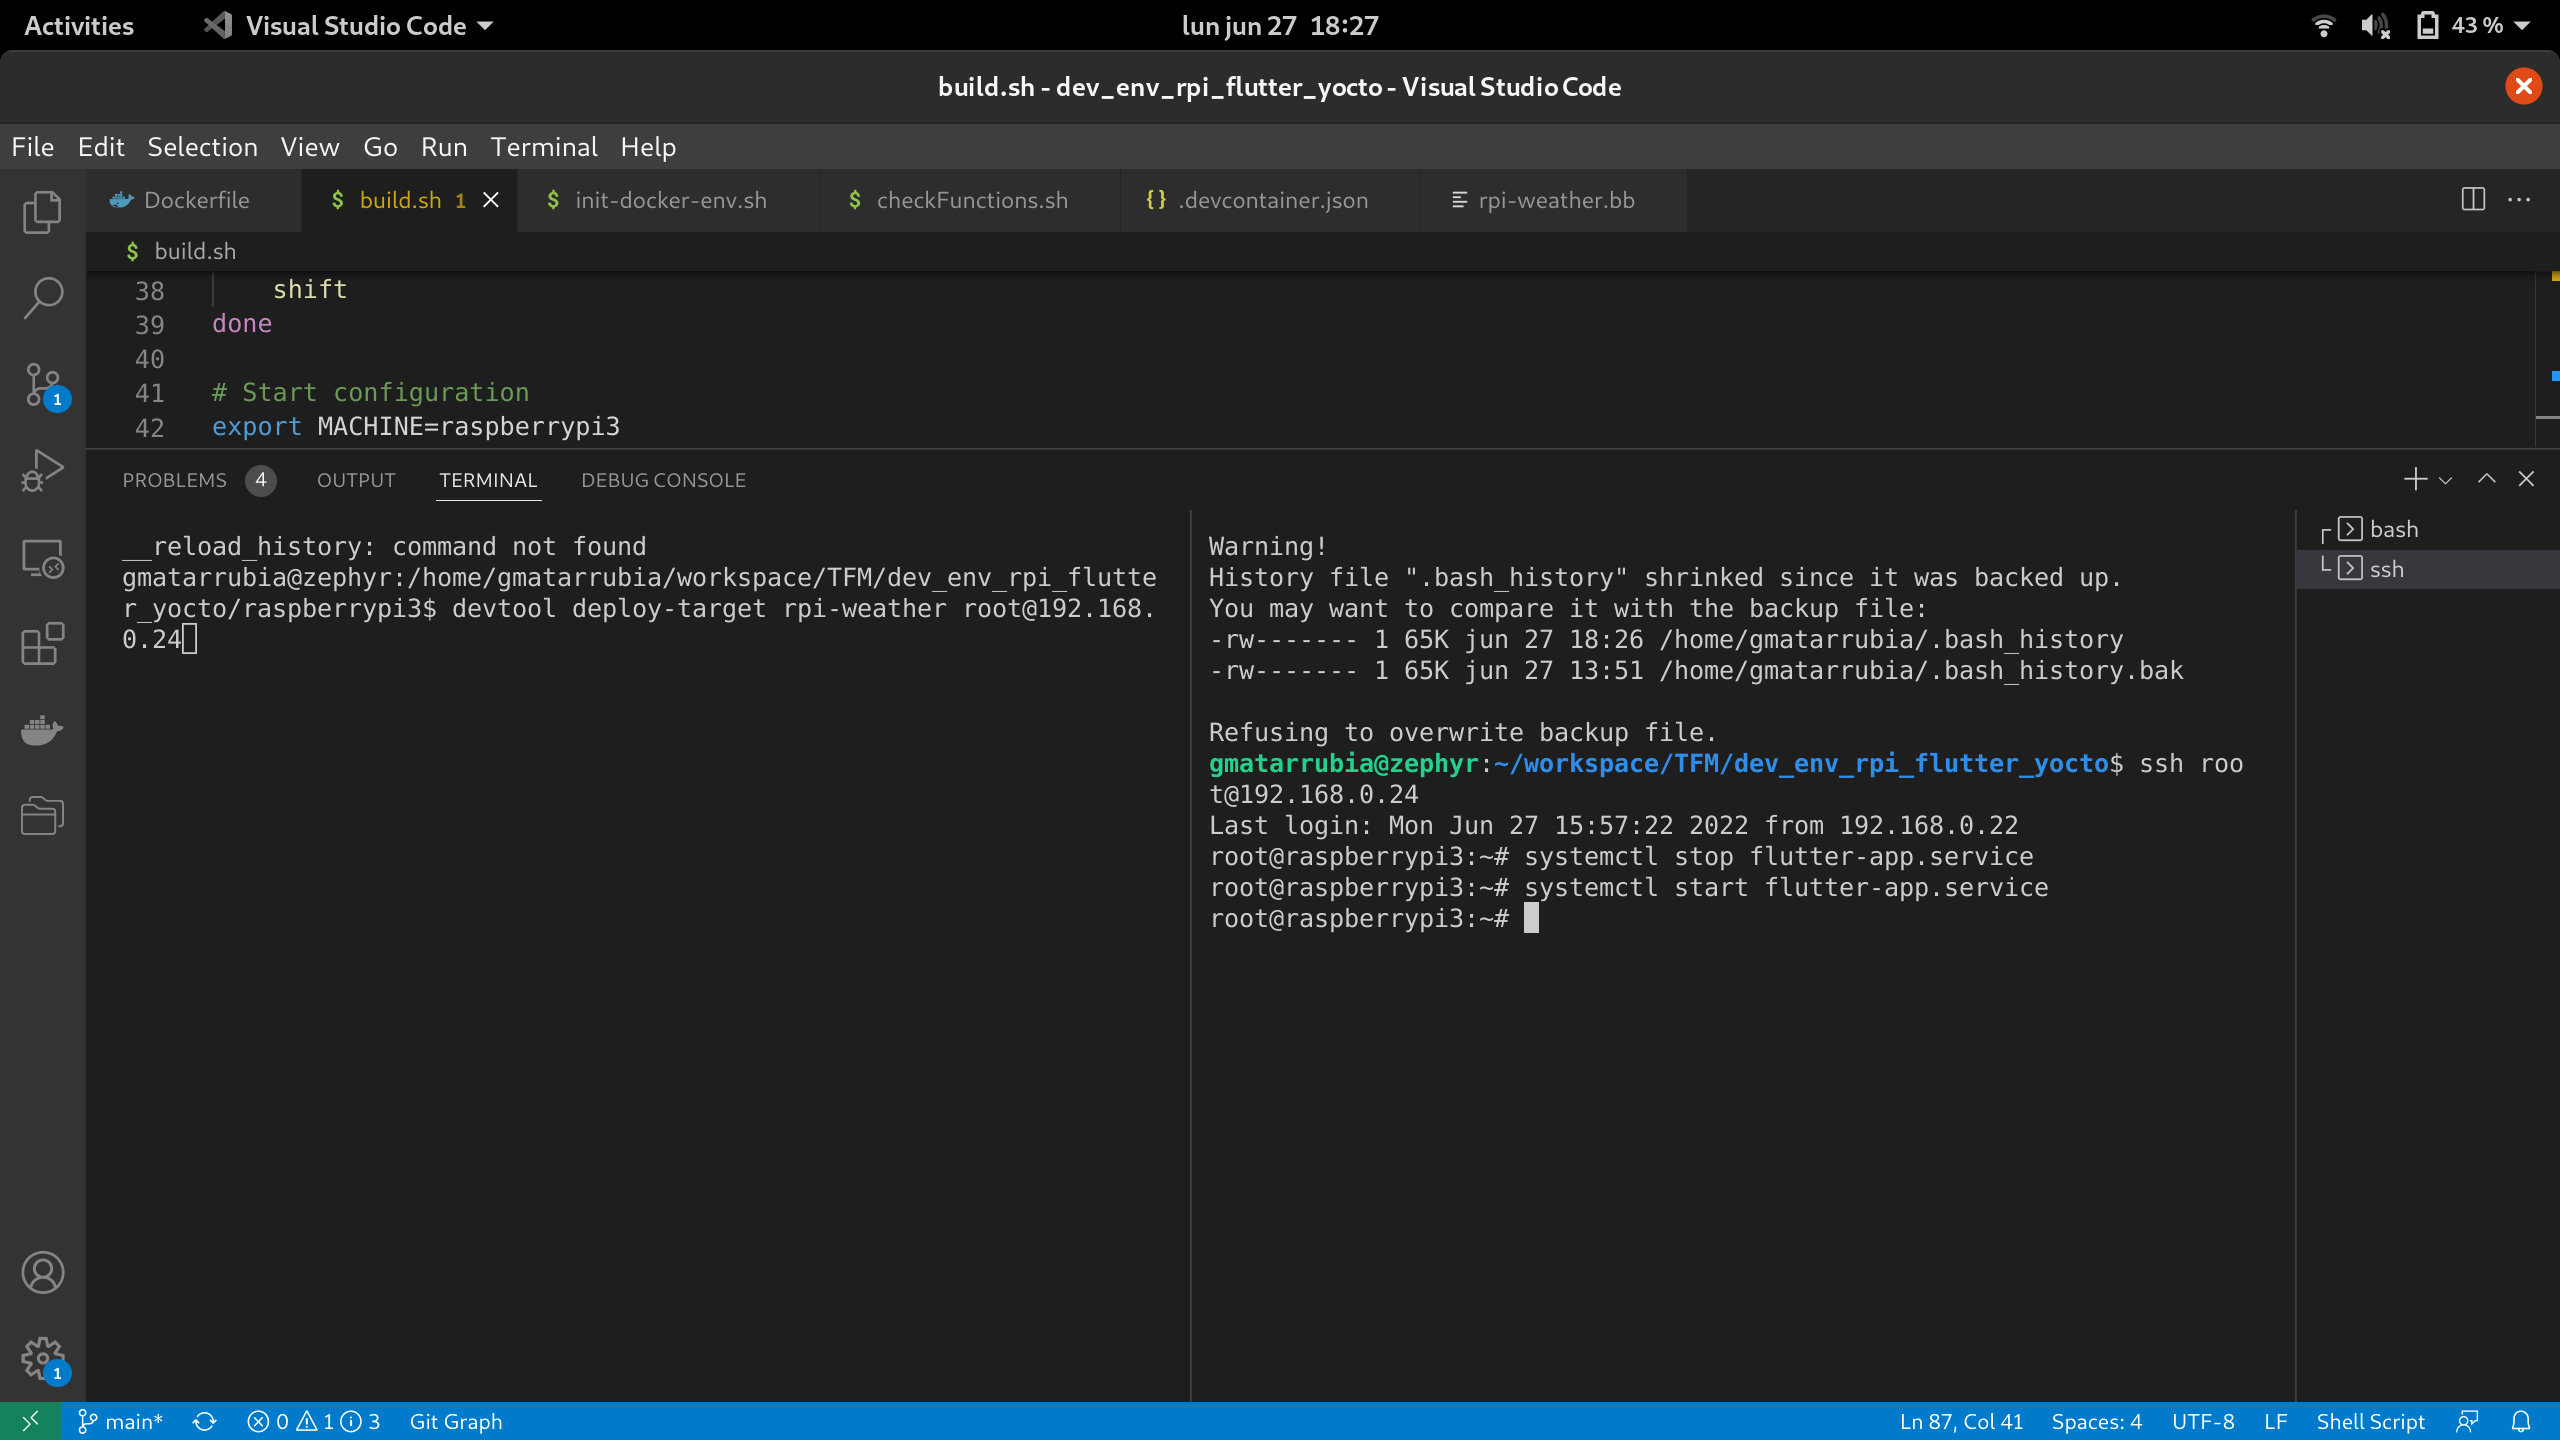
\includegraphics[width=0.95\textwidth]{imgs/dev3}
    \caption[Captura del despliegue.]{Captura del despliegue.}
    \label{imgs:deploy-target}
\end{figure}

\paragraph{}Una vez el despliegue se haya completado, volveremos a lanzar el servicio
de la aplicación flutter en la sesión ssh.

\begin{lstlisting}[style=consola, numbers=left]
    $ systemctl start flutter-app.service
\end{lstlisting}

\paragraph{}Ya estaríamos listos para probar en la aplicación en hardware. Cuando hayamos
realizado las pruebas pertinentes, será momento de confirmar los cambios en \gls{git}.

\begin{figure}[H]
    \centering
    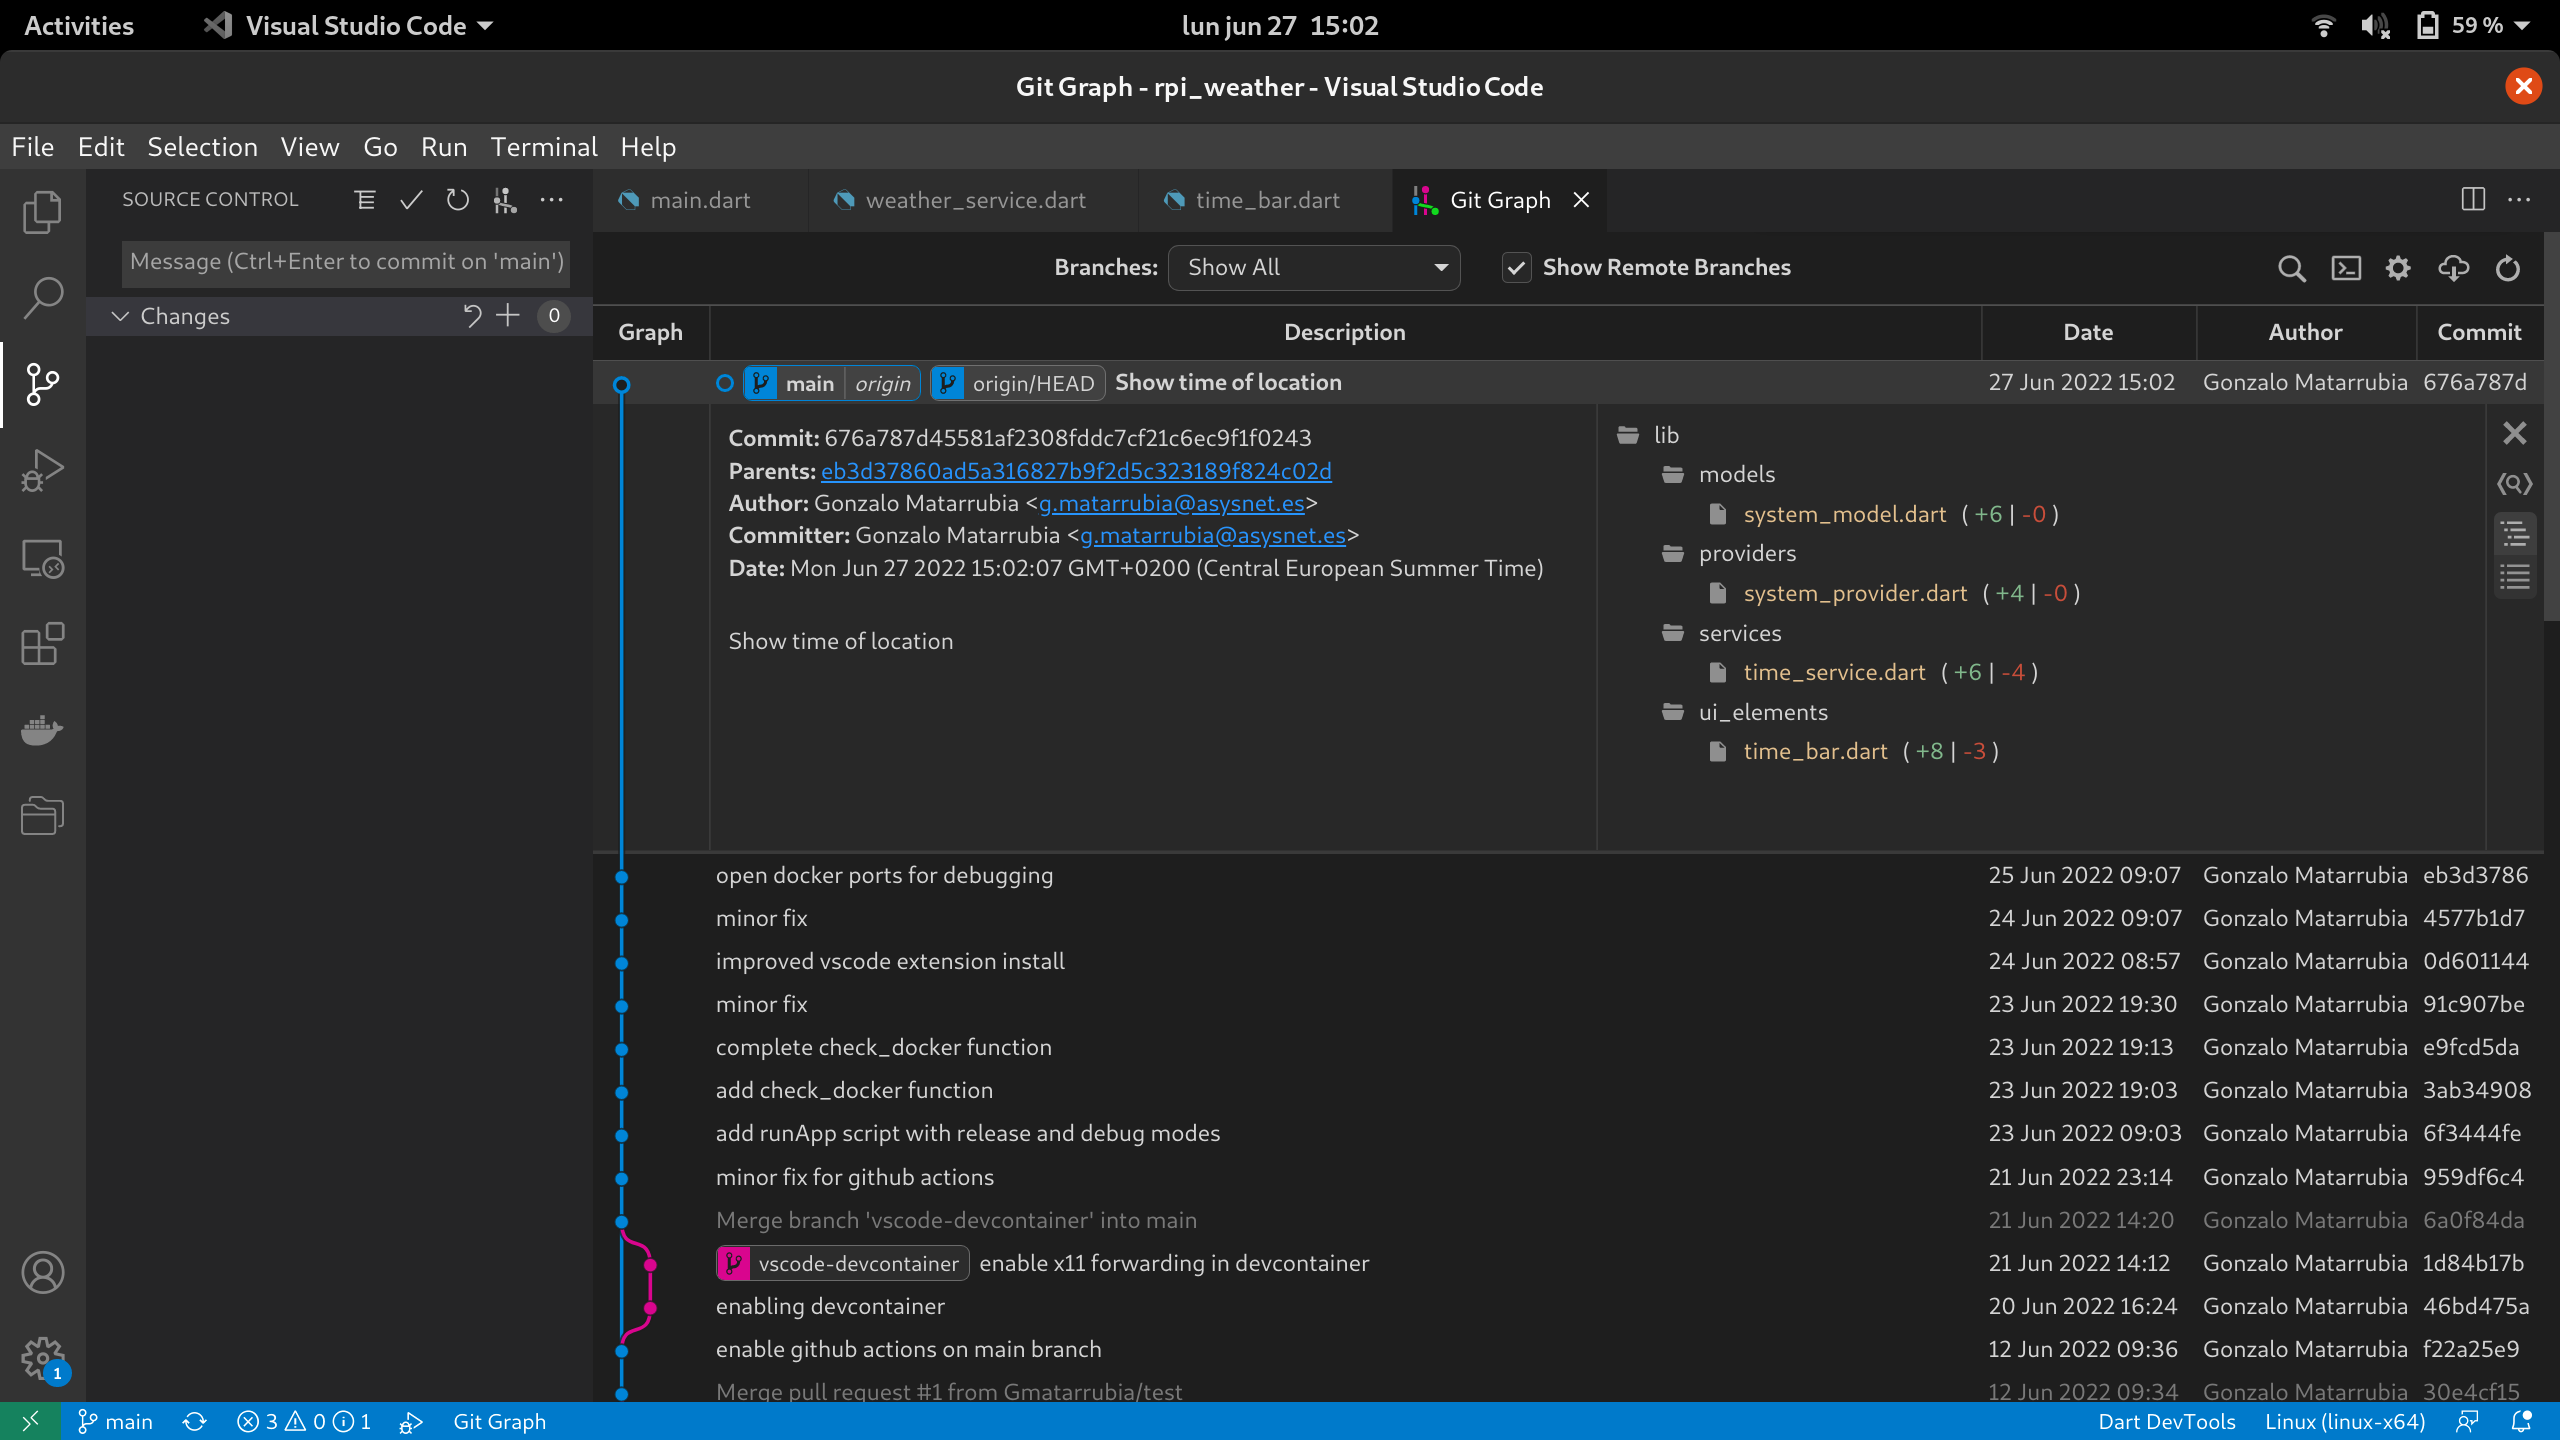
\includegraphics[width=0.95\textwidth]{imgs/dev2}
    \caption[Confimación de los cambios.]{Confimación de los cambios.}
    \label{imgs:commit}
\end{figure}

\paragraph{}Entonces, se ejecutarán los test unitarios de manera automatizada y nos
llegará un reporte en caso de fallo.

%las referencias a artículos se ponen con \cite,
%las referencias a glosario \gls,
%y las referencias a ecuaciones \eqref
%las referencias a imgenes, tablas o figuras o secciones
% se ponen con \ref (sólo número) o con \hyperref[sec:X]{text}